\documentclass[11pt]{article}

\usepackage{kernel_of_truth}
\usepackage{normal_setup}

\renewcommand{\R}{\mathbf{R}}

\begin{document}
\title{Math 2202 - Discussion 1 Quiz Solutions}
\author{Zachary Gardner}
\date{\texttt{zachary.gardner@bc.edu}}
\maketitle

\section*{Problem 1}
This problem is meant to help you explore what equations describe in the plane $\R^2$ compared to in $3$-dimensional space $\R^3$.
\begin{enum}{\alph}
\item What does the equation $x=4$ represent in the $xy$-plane, $\R^2$? What does it represent in $xyz$-space, $\R^3$? Illustrate with sketches.

\item What does the equation $y=3$ represent in $\R^3$? What does $z=5$ represent? What does the pair of equations $\{y=3,z=5\}$ represent? In other words, describe the set of points $(x,y,z)$ such that we have both $y=3$ and $z=5$. Illustrate with a sketch.

\item What does the set of three equations $\{x=4,y=5,z=3\}$ represent in $\R^3$? In other words, describe the set of points $(x,y,z)$ such that $x=4$, $y=5$, and $z=3$. Illustrate with a sketch.

\item Points are considered to be ``$0$-dimensional,'' lines are ``$1$-dimensional,'' planes are ``$2$-dimensional,'' and $\R^3$ is ``$3$-dimensional.'' Describe anything you notice about the relationship between the number of equations in $x,y,z$ and the dimension of the shape they represent in $\R^3$. Do the same thing for $\R^2$.
\end{enum}

\section*{Solution}
\begin{enum}{\alph}
\item In $\R^2$ the equation $x=4$ represents a vertical line. In $\R^3$ the equation $x=4$ represents a plane parallel to the $yz$-plane.

\item In $\R^3$ the equation $y=3$ represents a plane parallel to the $xz$-plane. Similarly, the equation $z=5$ represents a plane parallel to the $xy$-plane. The pair of equations $\{y=3,z=5\}$ represents the intersection of these two planes, which is a line parallel to the $x$-axis.

\item The set of three equations $\{x=4,y=5,z=3\}$ represents a single points in $\R^3$. This is because giving a point in $\R^3$ is the same as giving its coordinates.

\begin{figure}[ht]
\centering
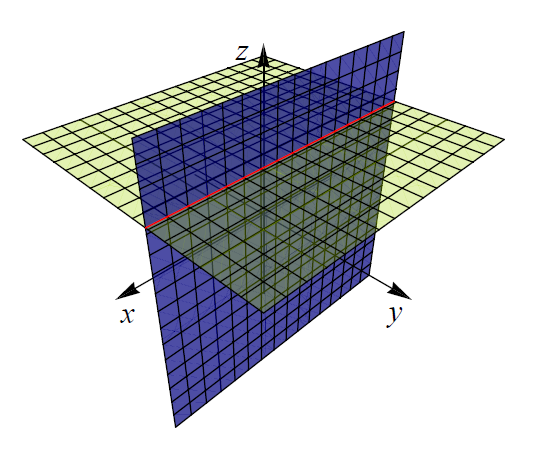
\includegraphics[scale=.5]{basic_plane_intersection}
\caption{Graph of the line $\{y=3,z=5\}$ in $\R^3$}
\end{figure}

\item In $\R^3$ it seems like the dimension of the shape described by a set of equations is three minus the number of equations. Similarly, in $\R^2$ it seems like the dimension of the shape described by a set of equations is two minus the number of equations. Loosely speaking, the codimension of an object in $\R^3$ is three minus the dimension. The codimension of an objection in $\R^2$ is two minus the dimension. Most of the time, the codimension is equal to the number of equations.
\end{enum}

\section*{Problem 2}
In this problem, you'll explore the set of points equidistant from two given points in $\R^3$. As you do, reflect back to what the set of points equidistant from two points in $\R^2$ is (Hint: high school geometry).
\begin{enum}{\alph}
\item Plot the points $(2,-1,5)$ and $(2,6,5)$. Write an equation for the set of points equidistant from $(2,1,5)$ and $(2,6,5)$ and simplify it as much as possible. Describe the set as specifically as possible. (Hint: Start with a generic point $(x,y,z)$. What would it mean for this point to be equidistant from the two given points? Write an equation to describe this.)

\item Plot the points $(2,-1,5)$ and $(3,6,0)$. Write an equation for the set of points equidistant
from $(2,-1,5)$ and $(3,6,0)$ and simplify it as much as possible. Describe the set as specifically as possible.
\end{enum}

\section*{Solution}
Intuitively, we expect the set of equidistant points to be something that ``cuts halfway'' between the two points. In $\R^2$, the set of points equidistant from two points is the perpendicular bisector, the line that bisects the line connecting the two points at a right angle. In $\R^3$ the same is true except that instead of just a line we get an entire plane as perpendicular bisector (if you have trouble seeing this then you might try playing around with a piece of paper).
\begin{enum}{\alph}
\item Let's first work intuitively. If we use the perpendicular bisector approach then the first thing to do is find the midpoint for $(2,-1,5)$ and $(2,6,5)$. Since both points have the same $x$- and $z$-coordinate we can find the midpoint just by averaging the $y$-coordinates, which gives $(2,5/2,5)$. From this we get the plane $y=5/2$. This approach is a solid argument but we still need to do a little more work to show that the set of all points equidistant from $(2,-1,5)$ and $(2,6,5)$ is exactly the plane $y=5/2$. To do this we use the distance formula. Say we pick a point $(x,y,z)$ floating ``randomly'' out in three-dimensional space. The distance from $(x,y,z)$ to $(2,-1,5)$ is 
$$\sqrt{(x-2)^2+(y+1)^2+(z-5)^2},$$
while the distance from $(x,y,z)$ to $(2,-1,5)$ is 
$$\sqrt{(x-2)^2+(y-6)^2+(z-5)^2}.$$
Setting these equal and squaring both sides gives
\begin{align*}
\textcolor{red}{(x-2)^2}+\textcolor{blue}{(y+1)^2}+\textcolor{green}{(z-5)^2}
=\textcolor{red}{(x-2)^2}+\textcolor{blue}{(y-6)^2}+\textcolor{green}{(z-5)^2}.
\end{align*}
Simplifying gives $(y+1)^2=(y-6)^2$ and thus $2y+1=-12y+36$, whose only solution is $y=5/2$.

\item We could first use the perpendicular bisector approach as we did earlier but this would be tricky since the $x$-, $y$-, and $z$-coordinates are all different. So, we instead use the distance formula. Again picking some random point $(x,y,z)$ in three-dimensional space, we have distances 
$$\sqrt{(x-2)^2+(y+1)^2+(z-5)^2}$$
and
$$\sqrt{(x-3)^2+(y-6)^2+z^2}.$$
Setting these equal, squaring, and simplifying gives the equation $2x+14y-10z=15$. Intuitively, we expected to get a plane and so it is natural to wonder if this is the equation of a plane. The answer, it turns out, is yes! One way of thinking about this is to view a plane as just a bunch of lines. For example, the $xy$-plane in $\R^3$ can be obtained by taking the $y$-axis and ``stretching it out'' infinitely in both directions along the $x$-axis. In other words, the $xy$-plane is just a bunch of translations of the $y$-axis. A general plane in $\R^3$ need not be parallel to one of the coordinate planes, but the general procedure of taking a line and stretching it out in both directions along some other line still works. From the equation $2x+14y-10z=15$ we can obtain a line on the plane by holding one of the variables $x,y,z$ fixed. For example, if we take $z=0$ then we are left with the equation $2x+14y=15$. This is the equation of a line in the $xy$-plane, which is the same as the plane $z=0$ (no coincidence!).
\end{enum}

\section*{Problem 3}
\textbf{What region is this in $\R^3$?} For each of the following, describe as fully as possible the region represented by the equation or set of equations. 
\begin{enum}{\alph}
\item $x=3,y=-7$

\item $y=2x+3$

\item $y=2x+3,z=5$

\item $y=3x+1,z=-2,x=y$

\item $x^2=3$

\item $x^2+y^2+z^2=3$

\item $y=x^2+3$

\item $x^2+z^2=3$

\item $y^2+2z^2=3$
\end{enum}
Here are some things to address and tips for thinking and visualizing:
\begin{itemize}
\item What is a geometric object?

\item What \emph{dimension} is it? Is it a line or curve? Is it $2$-dimensional line like a plane? For example, if you think ``cone'' then is it the surface of the cone (2D) or a solid cone (3D)? 

\item If the equation doesn't involve one of the variables (for example, there is no $z$ in the equation), what does that mean about the possible values of $z$ for points in the region? (A variable which does not have any restriction on it is sometimes called a \emph{free variable} or \emph{independent variable}.)

\item How does the region relate to the coordinate planes or axes? Is it parallel or perpendicular to any of them?

\item For some, it may be useful to think about whether the object intersects the coordinate planes. To test intersection with a coordinate plane (e.g., the $xy$-plane) we use the equation for that plane (e.g., $z=0$) and solve those equations together. We call such an intersection a \emph{trace} of the region. However, we still have to consider the equation in $\R^3$ -- what's the role of the other variable (e.g., $z$)?
\end{itemize}

\section*{Solution}
\begin{enum}{\alph}
\item This is a plane parallel to the $z$-axis.

\item This is a plane which is not parallel to any of the coordinate planes.

\item This is a line, obtained as the intersection of two planes.

\item We have $3x+1=x$ and so $x=-1/2$. Hence, $y=3(-1/2)+1=-1/2$ and so we get the point $(-1/2,-1/2,-2)$.

\item The equation $x^2=3$ forces $x=\pm\sqrt{3}$. Since $y,z$ can be anything, we get two parallel planes $x=-\sqrt{3}$ and $x=\sqrt{3}$.

\item This is the equation of a sphere centered at the origin $(0,0,0)$ with radius $\sqrt{3}$.

\item The equation $y=x^2+3$ describes a parabola in the $xy$-plane. Since $z$ can be anything we then stretch this parabola out infinitely in both directions along the $z$-axis.

\item The equation $x^2+z^2=3$ describes a circle in the $xz$-plane centered at $(0,0,0)$ with radius $\sqrt{3}$. Since $y$ can be anything we then stretch this circle out infinitely in both directions along the $y$-axis. In other words, we get a cylinder.

\item The equation $y^2+2z^2=3$ describes an ellipse in the $yz$-plane. Since $x$ can be anything we then stretch this circle out infinitely in both directions along the $x$-axis. In other words, we get an ``elliptic cylinder.''
\end{enum}

\section*{Problem 4}
(Exploratory) Another way to think about describing regions in $\R^2$, $\R^3$, and higher dimensions is in terms of a \emph{parametric equation}. For example, in $\R^2$, consider all points 
$$\ip{\cos t,\sin t}$$ 
where $t$ is any real value. What is this object? What about the following? 
$$\ip{2\cos t,\sin t}$$

\section*{Solution}
To understand the set of all points in $\R^2$ parametrized by $\ip{\cos t,\sin t}$, let $x=\cos t$ and $y=\sin t$. The famous trigonometric identity $\sin^2t+\cos^2t=1$ tells us that $x^2+y^2=1$ and so what we have is a circle. To understand the set of all points in $\R^2$ parametrized by $\ip{2\cos t,\sin t}$, we take a similar approach to before and let $x=2\cos t$ and $y=\sin t$. Then, $\cos t=x/2$ and so as before we have 
$$\paren{\df{x}{2}}^2+y^2=1.$$
This is the equation of an ellipse!
\end{document}